\section{Problem 3}
Changing the system matrix with state feedback.

The rotary mass-spring-damper system shown below has an input torque $u = T$ and
output position $\theta$ with a rotational spring $k_{\theta}$ and rotational damper $c_{\theta}$

\begin{figure}[htp]
    \centering
    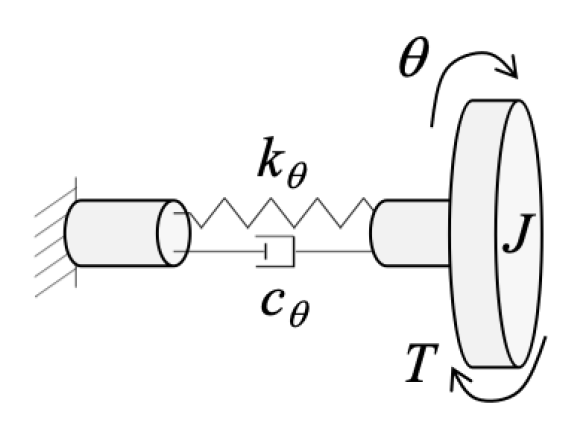
\includegraphics[width=6cm]{images/Q3.png}
\end{figure}

\subsection{a)}
Find the state space representation of this system.
\subsubsection{\textit{ Sol. }}

Define the state vector: $\textbf{x} = 
\begin{bmatrix}
    x_1\\
    x_2
\end{bmatrix} = 
\begin{bmatrix}
    \theta\\
    \dot{\theta}
\end{bmatrix}$, input $u = T$, and output $y = \theta$.

We can write the equation of motion as: $J\ddot{\theta} = - k_{\theta}\theta - c_{\theta}\dot{\theta} + T$ $\Rightarrow $   $\ddot{\theta} = - \frac{k_{\theta}}{J}\theta - \frac{c_{\theta}}{J}\dot{\theta} + \frac{1}{J}T$

\begin{equation} \label{eq:9}
    \begin{aligned} 
        \dot{\textbf{x}} &= 
        \begin{bmatrix}
            0 & 1 \\
            -\frac{k_{\theta}}{J} & -\frac{c_{\theta}}{J}
        \end{bmatrix}
        \textbf{x} + 
        \begin{bmatrix}
            0\\
            \frac{1}{J}
        \end{bmatrix}
        u
        \\
        \dot{y} &=
        \begin{bmatrix}
            1 & 0
        \end{bmatrix}
        \textbf{x} + 
        \begin{bmatrix}
            0
        \end{bmatrix}
        u
    \end{aligned}
\end{equation}



\subsection{b)}
Now assume that your input torque $T$ is a function of the system state so that
$T = R - \textbf{k}\textbf{x}$ where $\textbf{k}$ is a vector $\begin{bmatrix}k_1 & k_2\end{bmatrix}$ and $\textbf{x}$ is the state vector. Find the new state equation assuming a new input, $u = R$.

\subsubsection{\textit{ Sol. }}

Substitute $u$ in Eq.\ref{eq:9} with 
$\left(R - \begin{bmatrix} k_1 & k_2 \end{bmatrix} \textbf{x}\right)$ we get:

\begin{equation}
    \begin{split}
        \dot{\textbf{x}} &= 
        \begin{bmatrix}
            0 & 1 \\
            -\frac{k_{\theta}}{J} & -\frac{c_{\theta}}{J}
        \end{bmatrix}
        \textbf{x} + 
        \begin{bmatrix}
            0\\
            \frac{1}{J}
        \end{bmatrix}
        \left(R - \begin{bmatrix} k_1 & k_2 \end{bmatrix}
        \textbf{x}
        \right) \\
        &= 
        \left(\begin{bmatrix}
            0 & 1 \\
            -\frac{k_{\theta}}{J} & -\frac{c_{\theta}}{J}
        \end{bmatrix} - \begin{bmatrix}
            0\\
            \frac{1}{J}
        \end{bmatrix}\begin{bmatrix}
            k_1 & k_2
        \end{bmatrix}\right)
        \textbf{x} + 
        \begin{bmatrix}
            0\\
            \frac{1}{J}
        \end{bmatrix}R
        \\
        &= 
        \begin{bmatrix}
            0 & 1 \\
            -\frac{k_{\theta} + k_1}{J}& -\frac{c_{\theta} +k_2}{J}
        \end{bmatrix}
        \textbf{x} + 
        \begin{bmatrix}
            0\\
            \frac{1}{J}
        \end{bmatrix}R\\
        &= 
        \begin{bmatrix}
            0 & 1 \\
            -\frac{k_{\theta} + k_1}{J}& -\frac{c_{\theta} +k_2}{J}
        \end{bmatrix}
        \textbf{x} + 
        \begin{bmatrix}
            0\\
            \frac{1}{J}
        \end{bmatrix}u\\ 
        \dot{y} &=
        \begin{bmatrix}
            1 & 0
        \end{bmatrix}
        \textbf{x} + 
        \begin{bmatrix}
            0
        \end{bmatrix}
        \left(R - \begin{bmatrix} k_1 & k_2 \end{bmatrix}
        \textbf{x}
        \right) \\
        &= \begin{bmatrix}
            1 & 0
        \end{bmatrix}
        \textbf{x} + 
        \begin{bmatrix}
            0
        \end{bmatrix}u
    \end{split}
\end{equation}

\subsection{c)}
Assuming $J = 1\ kg\cdot m^2$, $c_{\theta} =2\ N\cdot m\cdot s/rad$, $k_{\theta} =5\ N\cdot m/rad$, simulate the response to a step input of $0.1\ N\cdot m$ for the original system and a step of $0.64\ N\cdot m$ for the new system with $k =\begin{bmatrix}27 & 6\end{bmatrix}$.

\subsubsection{\textit{ Sol. }}
Matlab code:
\lstinputlisting{codes/Question3c.m}
Result:
\begin{figure}[htp]
    \centering
    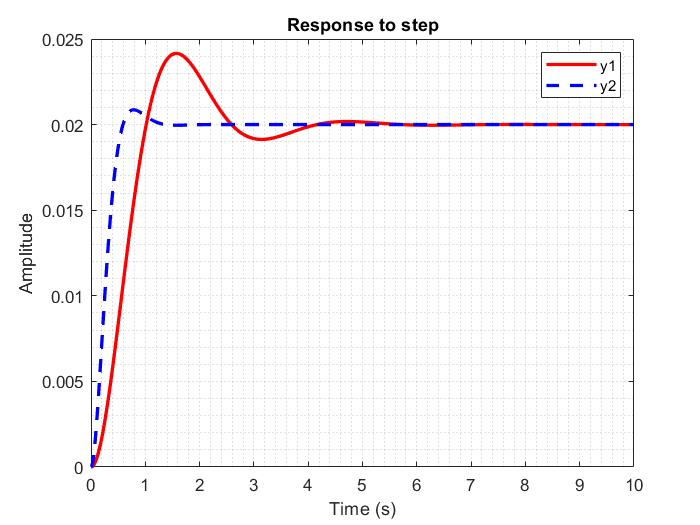
\includegraphics[width=15cm]{images/Q3_c_fig.png}
    \caption{Step Response}
    \label{fig:Q3c}
\end{figure}
\pagebreak